\documentclass{standalone}
\usepackage{tikz,pgfplots,xparse,xfp}
\usetikzlibrary{fit,arrows,calc,positioning,matrix,external,patterns}
\pgfplotsset{compat=1.16}
\thispagestyle{empty}
%creates define variables function
  \ExplSyntaxOn
  \NewDocumentCommand{\definevar}{mm}{\cs_new:Npx #1 {\fp_eval:n { #2 }}}
  \ExplSyntaxOff
%
% define variables
% define probability and delta
	\newcommand{\prelecalpha}{0.35} % adjust parameter alpha for prelec here
	%adjust parameter beta for prelec here
	\newcommand{\prelecbetaone}{3}
	\newcommand{\prelecbetatwo}{1} 
	\newcommand{\prelecbetathree}{1.5} 
	\newcommand{\prelecbetafour}{2} 	
%define Prelec function (p=no.1,alpha=no.2,beta=no.3)
	\newcommand{\prelec}[3]{exp((-#3)*((-ln(#1))^(#2)))}
%The scale of the graphic can be changed here (units = cm)
	\newcommand{\xscale}{10}
	\newcommand{\yscale}{10}
%
\begin{document}
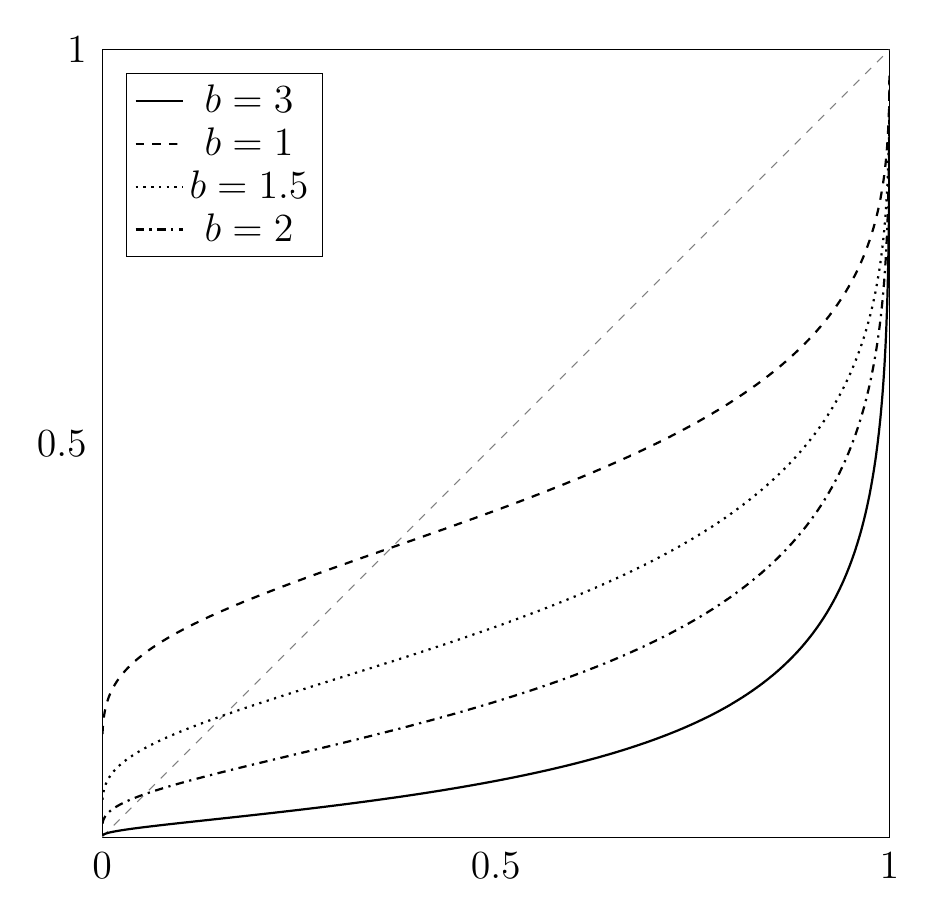
\begin{tikzpicture} %alternatively with color (right graphic)
  \tikzstyle{every node}=[font=\Large]
  %draw marks
  \draw [-] (0,0) -- (0,0) node[below, yshift=-2pt] {$0$};
  \draw [-] (\xscale*0.5,0) -- (\xscale*0.5,0) node[below, yshift=-2pt] {$0.5$};
  \draw [-] (\xscale,0) -- (\xscale,0) node[below, yshift=-2pt] {$1$};
  \draw [-] (0,\yscale*0.5) -- (0,\yscale*0.5) node[left,xshift=-2pt] {$0.5$};
  \draw [-] (0,\yscale) -- (0,\yscale) node[left,xshift=-2pt] {$1$};
  %draw functions
  \begin{axis}[domain=0:1, smooth, xmin=0, xmax=1, ymin=0, ymax=1, width=\xscale cm, height=\yscale cm, scale only axis=true, ticks=none, legend pos=north west] %This sets up a new axis environment
    \addplot [samples=3,dashed,color=gray, forget plot] {x}; %Diagonal
    \addplot [samples=2000,thick, forget plot] {\prelec{x}{\prelecalpha}{\prelecbetaone}};
    \addplot [samples=2000,thick,dashed,forget plot] {\prelec{x}{\prelecalpha}{\prelecbetatwo}};
    \addplot [samples=2000,thick,dotted,forget plot] {\prelec{x}{\prelecalpha}{\prelecbetathree}};
    \addplot [samples=2000,thick,dash dot,forget plot] {\prelec{x}{\prelecalpha}{\prelecbetafour}};
    %legend
    \addlegendentry{$b=\prelecbetaone$}
    \addlegendimage{thick}
    \addlegendentry{$b=\prelecbetatwo$}
    \addlegendimage{thick,dashed}
    \addlegendentry{$b=\prelecbetathree$}
    \addlegendimage{thick,dotted}
    \addlegendentry{$b=\prelecbetafour$}
    \addlegendimage{thick,dash dot}
    %		\addlegendentry{$w(p)=e^{-\prelecbeta(-ln(p))^{\prelecalpha}}$}
    %		\addlegendimage{no markers,black}
    %		\addlegendentry{} %This adds an empty line in the legend for a better fit
    %		\addlegendimage{empty legend}
  \end{axis}
\end{tikzpicture}
\end{document}